\documentclass{article}

\usepackage{proposal}

\setproposaltitle{Composing Sparsity in Match-LSTM for Machine Comprehension}

\addauthor{Saransh Bhatnagar}{150637}
\addauthor{Siddhant Garg}{150711}
\addauthor{Divyansh Singhvi}{150238}
\addauthor{Megha Agarwal}{150403}
\addauthor{Dushyant Kumar}{150242}

\begin{document}
\makeheader

\rabstract{
	Machine Comprehension is a fundamental problem in Natural Language.
	There are many datasets which provide wide range of corpus for this task.
	We intend to explore the most recently released dataset, the Stanford Question Answering Dataset \citep[SQuAD,][]{squad}, which offers a large number of real crowdsourced questions and passages.
	We try to explore a number of approaches to this task, particulary Match-LSTMS along with PointerNets, as proposed by \cite{match-lstm-mc} for the task of machine comprehension.
	Or main goal is to improve the scalability of the models by targetting the sparsity of the learned networks in an attempt to reduce the hypothesis space of our model, while trying to minimize loss of accuracy.
}

\begin{psection}{Introduction}

	\sloppy
	Question Answering (or Machine Comprehension) is a fundamental problem in Natural Language Processing where we want the computer system to be able to understand a corpus of human knowledge and answer questions provided in Natural Language.
	This involves seemingly simple, but complex tasks such as understanding human language enough to interpret provided questions, and searching for an appropriate answer.

	A distinguishing characteristic between humans and naive models is the ability of humans to quickly relate the passages to focus on subsets of the passage with demarcating words related to the task at hand.
	There exists many approaches to this problem.

	There have been many approaches to solving the machine comprehension, however most lack the scalability and the lightness of the model. In our project, we intend to explore the high maintenance characteristic of these models, and attempt to apply sparsity inducing techniques in order to reduce the heaviness of the models.

\end{psection}

\begin{psection}{Problem Statement}

	In this course project, we aim to explore the problem of Machine Comprehension (or Question Answering) by using Deep Learning based models and see how they perform on the Stanford Question Answering Dataset (SQuaD).

	We state our problem statement similar to as stated in \citep{squad}.

	For each question-passage-answer tuple $(\vQ, \vP, \vA)$, where $\vQ = (q_1 \dots q_M)$ are the tokens for the question, $\vP = (p_1 \dots p_N)$ are the tokens for the passage, and $\vA = (a_b, a_e)$ is the answer span, $a_b$ and $a_e$ representing the beginning and ending indices in the passage.
	The task is maximising the conditional probability $\prob{\vA = (a_b, a_e) \pipe \vQ, \vP}$, \ie the probability of answer being correct, given the question and the passage or instead estimating $\prob{\vA \pipe \vQ, \vP}$ and thereby finding the answer
	\begin{align*}
		\vA^\ast = \argmax{\vA} \prob{\vA \pipe \vQ, \vP}.
	\end{align*}

\end{psection}

\begin{psection}{Dataset}

	We will use the SQuad \citep{squad} dataset, for the goal of studying techniques in Machine Comprehension.

	The Stanford Question Answering Dataset (SQuAD) is a reading comprehension consisting of 100,000+ question-answers corresponding to passages extracted from over 500 wikipedia articles, where the answer to each question is a continuous segment of text from that passage.

	The dataset is roughly portioned in 80k test set, 10k training set and 10k validation set.
	SQuAD does not provide a list of answer choices for each question, as compared to other datasets.
	Also, unlike some other contemporary datasets whose questions and answers are created automatically in cloze style, the question and answers in SQUAD were created by humans through crowdsourcing making the dataset more realistic.

	Another difference between SQUAD and cloze style queries is that answers to cloze style queries are single words or entities while answer in SQAD can be non-entities and can contain long phrase.

	The squad dataset has a varied length of questions although most of them lie in the 5-15 word range.
	The context length is mostly distributed (evenly) between 20 -- 250 word range.
	The variety of the context length, makes fitting to some piece of the context difficult, which is a good characteristic of the dataset.

	In additon, the span-based QA setting is quite natural.
	For many user questons into search engines, open-domain QA systems are often able to find the right documents that contain the answer.
	The challenge is the last step of ``answer extracton'', which is to find the shortest segment of text in the passage or document that answers the question \footnote{\url{https://rajpurkar.github.io/mlx/qa-and-squad/}}.

\end{psection}

\begin{psection}{Relevant Background}

	\begin{psubsection}{Long Short Term Memory}
		Long Short Term Memory \citep[LSTM,][]{lstm} networks are a special kind of Recurrent Neural Networks (RNNs), capable of learning long-term dependencies.
		LSTMs are explicitly designed to avoid long-term dependency problem, for example, for predicting a word after observing a sequence of words history, we might need the context of the words observed much before the `to be predicted' word.

		\sloppy 
		This requires a memory model, which vanilla RNNs are incapable of handling. Remembering information for long periods of time is default behavior of the LSTM networks, which is handled using states and the controlling the flow of information is handled using gating networks. LSTMs, therefore, have the ability to remove or add information to the cell state, regulated by gates or gated networks. The structure of a simple LSTM network is given in Figure \ref{fig:lstm}

		\begin{figure}[ht!]
			\centering
			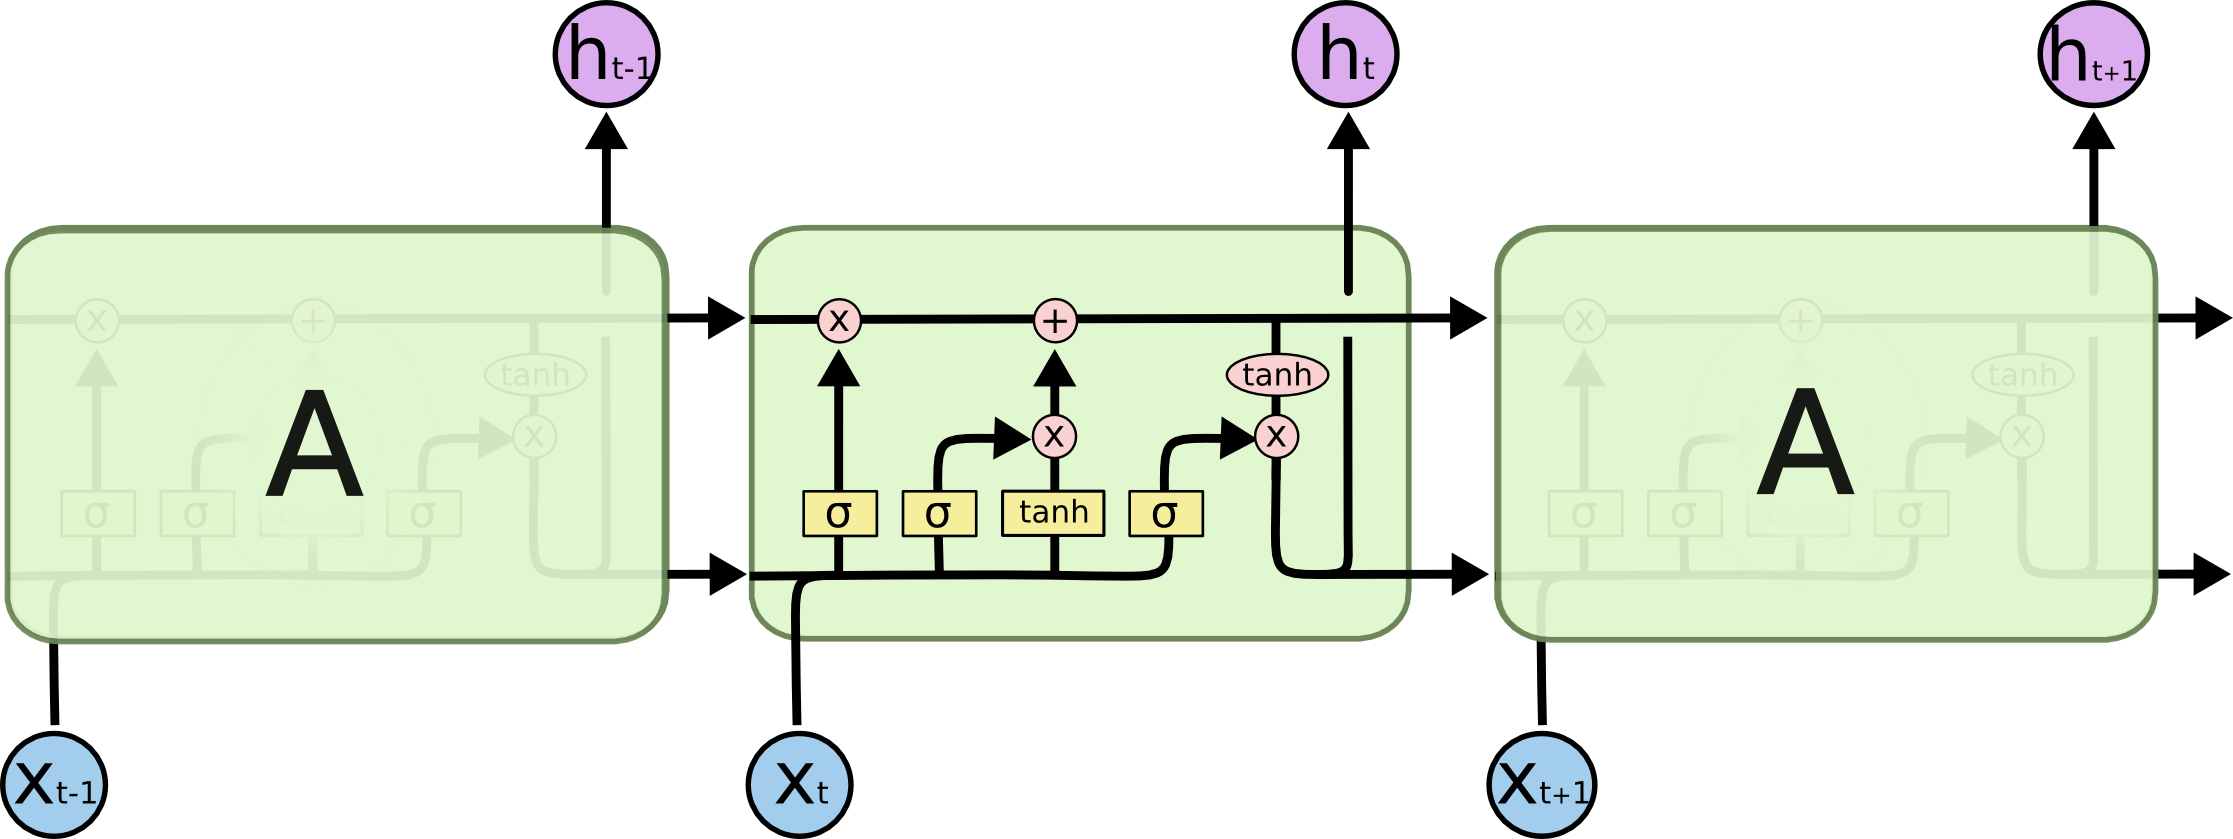
\includegraphics[width=0.8\textwidth]{includes/lstm-chain.png}
			\caption{Insides of a LSTM Network. \et{\citep[Source:][]{lstm-blog}}}
			\label{fig:lstm}
		\end{figure}

		\note{For the further discussion, we borrow the notations and description from \cite{lstm-blog}}

		\begin{pssubsection}{Layers of a LSTM}
			We define the state of the LSTM at a time state $t$ as $C_t$. A LSTM as described above consists of four layers that we describe as below.
			\begin{enumerate}[label=\bt{\theenumi.}]
				\ditem[Forget Gate Layer]
					\et{Forget Layer} decides what information we are going to throw away from cell by looking at previous cell state and the current data point (or word for the task of machine comprehension). The forget layer uses a sigmoid function to determine the amound of information to pass or to forget. The computed vector (or matrix) is represented by $f_t$

				\ditem[Input Gate Layer]
					What new information we are going to store in the cell state is decided by a sigmoid and a tanh layer.
					Sigmoid layer called the \et{input gate layer} decides which values we'll update, and to what extent, and the tanh layer creates a vector of new candidate values, $\widetilde{C}_t$, that will be added to the state.

				\ditem[Update Layer]
					Updation of the state is carried out by multiplying the old state $C_{t - 1}$ by $f_t$, the output from the forget layer, and adding the update values $\widetilde{C}_t$ to get the new state, \ie $C_t$.

				\ditem[Ouput Layer]
					The \et{Output Layer} handles the updation of the output label, using the new state, the input data and the old label.
					First, a sigmoid layer is run throuth the \et{concatenation} of the old label $h_{t - 1}$ and the data point.
					Then, the current (updated) cell state is passed through a tanh layer and multiplied to the output of the sigmoid gate to get the new label / output $h_t$.
			\end{enumerate}

			A detailed look at the states of the LSTM is given in Figure \ref{fig:lstm-flow}.
		\end{pssubsection}

		\begin{figure}[ht!]
			\centering
			\begin{minipage}{0.47\textwidth}
				\centering
				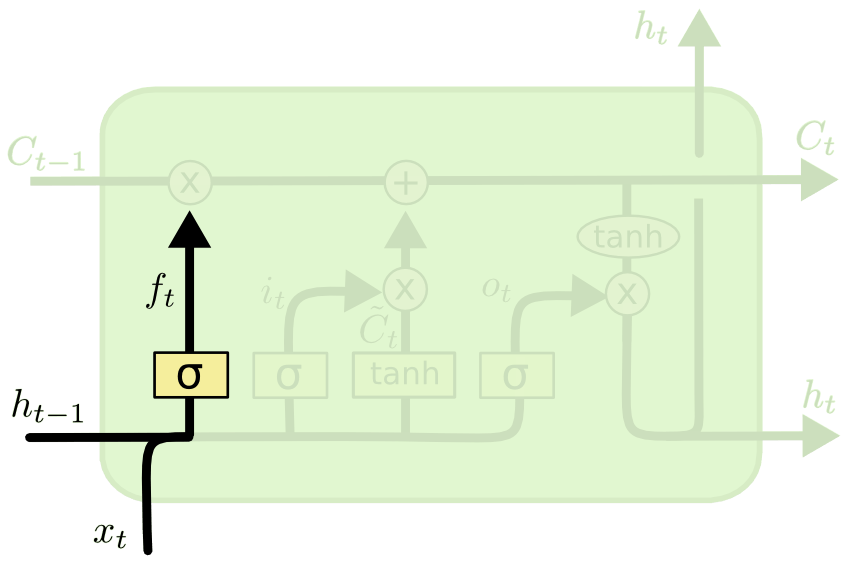
\includegraphics[height=135px]{includes/lstm1.png}
				\caption*{Forget Gate}
			\end{minipage}
			\begin{minipage}{0.47\textwidth}
				\centering
				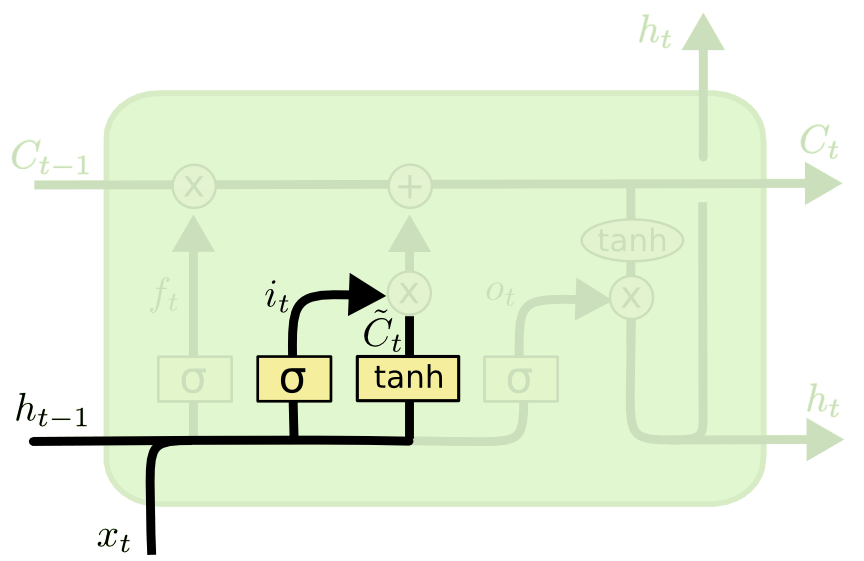
\includegraphics[height=135px]{includes/lstm2.png}
				\caption*{Input Gate}
			\end{minipage}
			\begin{minipage}{0.47\textwidth}
				\centering
				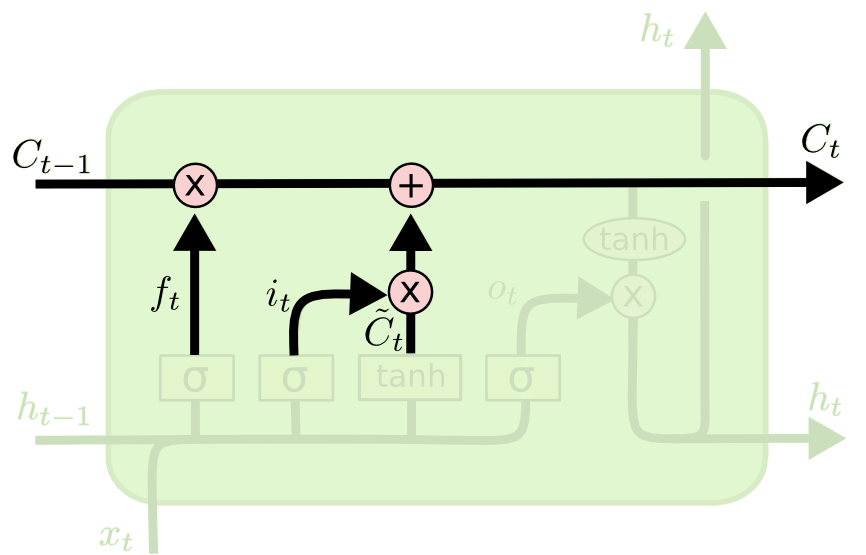
\includegraphics[height=135px]{includes/lstm3.png}
				\caption*{Value Updates}
			\end{minipage}
			\begin{minipage}{0.47\textwidth}
				\centering
				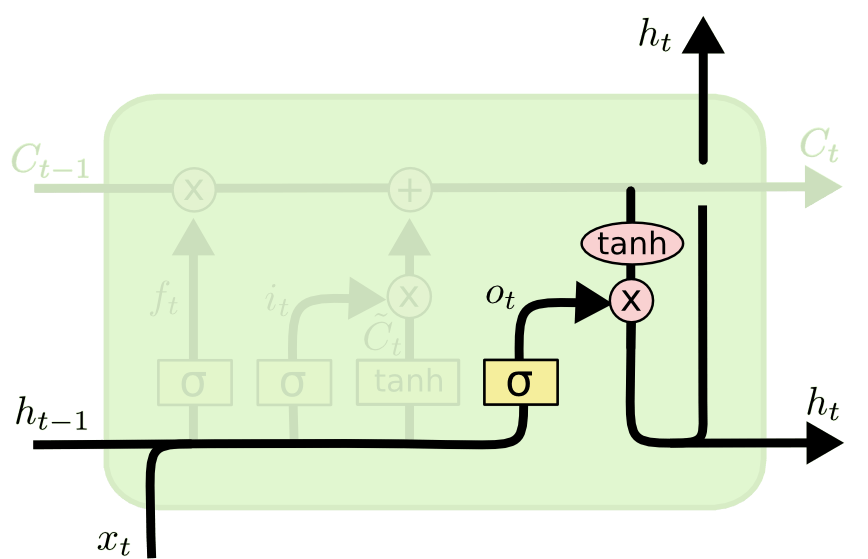
\includegraphics[height=135px]{includes/lstm4.png}
				\caption*{Output Layer}
			\end{minipage}
			\caption{Working of a simple LSTM. \et{\citep[Source:][]{lstm-blog}}}
			\label{fig:lstm-flow}
		\end{figure}

		\begin{pssubsection}{Bidirectional LSTMs}
			Bidirectional RNNs \citep[BRNNs,][]{rnn-blog}, which are the base of bidirectional LSTMs, are based on the idea that the output at time $t$ may not only depend on the previous elements in the sequence, but also future elements, for example, word prediction, such as filling in a blank within a sentence, might benefit from including the post blank words into consideration while prediction the current word.

			Bidirectional RNNs, in their essence, are just two RNNs stacked on top of each other.
			The output is then computed based on the hidden state of both RNNs.
			Combing BRNNs with LSTM gives bidirectional LSTM which can access long-range context in both input directions.

			\begin{figure}[ht!]
				\begin{minipage}{0.47\textwidth}
					\centering
					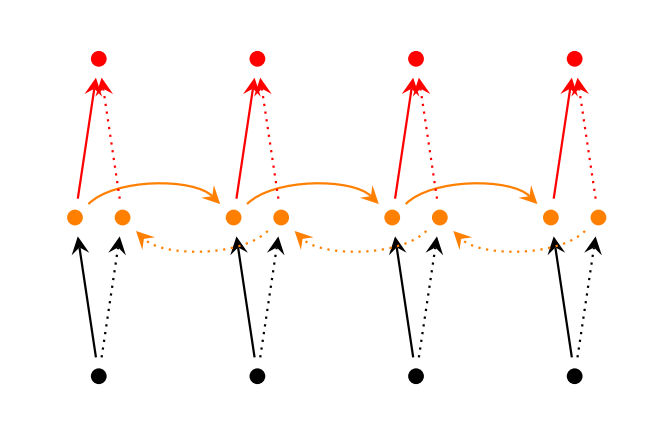
\includegraphics[width=200px]{includes/bidirectional-rnn.png}
					\caption*{(a) Bidirectional RNN}
				\end{minipage}
				\begin{minipage}{0.47\textwidth}

					\centering
					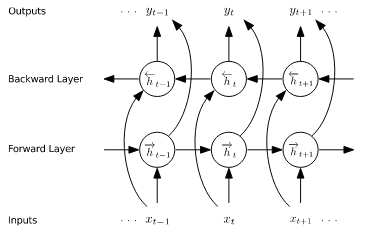
\includegraphics[width=200px]{includes/bidirectional-lstm.png}
					\caption*{(b) Bidirectional LSTM}
				\end{minipage}
				\caption{Biderectional RNNs (left) and LSTMs (right) \et{\citep[Source:][]{rnn-blog}}}
			\end{figure}

		\end{pssubsection}

		\begin{pssubsection}{Match-LSTMs}

			Match-LSTMs \citep{match-lstm} are an extension to basic LSTMs, introduced by \et{Wang and Jiang} for the purpose of textual entailment, and later used the same in machine comprehension to achieve state-of-the-art results on the SQuAD (at the time of publication).

			Match-LSTM attempts to recover an sequence of positions within a context paragraph using the contents of the context and an associated question \citep{match-lstm-m}.

			To verify textual entailment, match-LSTM goes through the tokens of the hypothesis sequentially. And for each position, attention mechanism is used to obtain a weighted vector representation of the premise. This weighted premise combined with current token of hypothesis fed into match-LSTM.

			\sloppy
			The match-LSTM model essentially sequentially aggregates the matching of the attention weighted premise to each token of the hypothesis and uses the aggregated matching result to make a final prediction.

			Details of the model are given in the papers \cite{match-lstm} and \cite{match-lstm-mc}

		\end{pssubsection}

	\end{psubsection}

\end{psection}

\begin{psection}{Previous Works}

	Traditional solutions question answering tasks relied on NLP pipelines that involved multiple steps of linguistic and lexical analysis, including syntactic parsing, named entity recognition, question classification, semantic parsing, etc.
	In these approaches each layer of parsing added its own set of errors or loss which propogated over pipelines to subtle failures that required a lot of manual tweaking to get to the right results.

	Existing end-to-end neural models assume that the answer is a single token making them unsuitable for use in SQuAD, which expects a sequence based answers. Hence, we require new and more advanced models for machine comprehension tasks. We have described a few of them below.

	Most of the state-of-the-art approaches have the following settings in common, which we, as well, will extend in our approach as an attempt to solve the problem of question answering in SQuAD.

	\begin{enumerate}
		\item Pre trained GLoVe \citep{glove} vectors are used as embeddings for each word, therefore formign the word embedding layer.

		\item This word embedding layer is connected through LSTM which could of different types like vanilla LSTM, bidirectional LSTM, match-LSTM, etc. to develop a context based embedding layer.

		\item \sloppy
		    This layer is followed by attention flow layer which is used to make the model aware of the query.
			The paragraph and query are both processed through the attention mechanism to generate an interdependent context, therefore learning a query aware latent representing of the passage.

		\item This latent representation is therefore used to predict the answer spans using various strategies, some of which we discuss briefly in the following sections.
	\end{enumerate}

	\begin{psubsection}{Bi-Directional Attention Flow for Machine Comprehension}

		The BiDAF \citep{bidaf} model is a hierarchical multi-stage process which consists of six layers. The comprehensive model is given in Figure \ref{fig:bidaf}.

		\begin{enumerate}[label=\bt{\theenumi.}]
			\ditem[Character Embedding Layer.] Character embedding layer is responsible for mapping each word to a high-dimensional vector space.
			We obtain the character-level embedding of each word using Convolutional Neural Networks (CNN) \citep{Char_embedding}.

			\ditem[Word Embedding Layer.] Word embedding layer also maps each word to a high-dimensional vector space.
			Pre-trained GloVe vectors, are used to obtain the fixed word embedding of each word.

			\ditem[Contextual Embedding Layer.] This layer model the temporal interactions between words.
			For this, LSTM is placed in both directions and concatenate the outputs of the two LSTMs, thus obtaining \bt{H} from context word vectors $\vX$ and $\vU$ from query word vectors $\vQ$.

			\ditem[Attention Flow Layer.] Attention flow layer is responsible for linking information from context and query words.
			The inputs to the layer are contextual vector representations of the context $\vH$ and the query $\vU$.
			The outputs of the layer are the query-aware vector representations of the context words, $\vG$, along with the contextual embeddings from the previous layer. Shared similarity matrix, $\vS$ is used to obtain the attentions and the attended vectors in both direction.

			The similarity matrix $\vS$ is used to obtain the attentions and the attended vectors in both direction, \ie \et{Context-to-Query} Attention and \et{Query-to-Context} Attention.

			\ditem[Modeling Layer.] The input to the modeling layer is $\vG$, which encodes the query-aware representations of context words by using two layered bi-directional LSTM.

			The output of the modeling layer captures the interaction among the context words conditioned on the query.
			The output of the modelling layer is $\vM$.

			\ditem[Output Layer.] This layer predict the start and the end indices of the phrase in the paragraph to answer the query.
			It outputs probability distribution of the start index, $p^1$ over the entire paragraph by using $\vG$ and $\vM$ and predicts the probability distribution of the end index, $p^2$ by using $\vG$ and $M^{2}$, where $M^{2}$ is calculated by passing $\vM$ through another bidirectional LSTM.

		\end{enumerate}

		\begin{figure}[ht!]
			\centering
			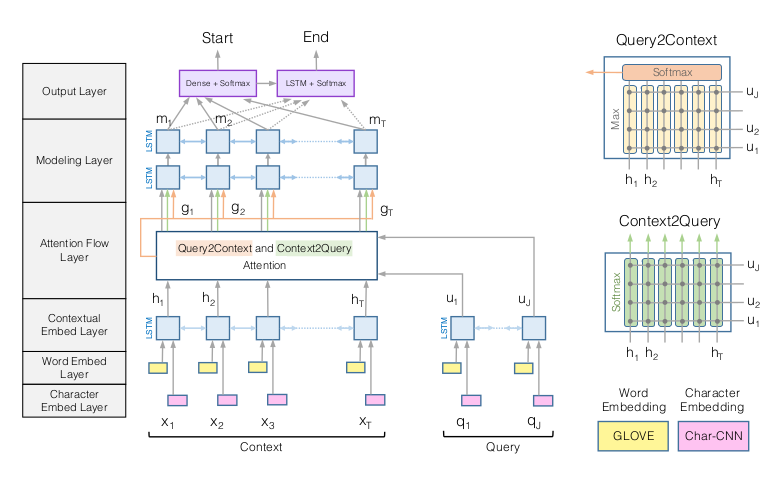
\includegraphics[height=250px]{includes/bidaf.png}
			\caption{Bi-Direction Attention Flow Model \et{\citep[Source:][]{bidaf}}}
			\label{fig:bidaf}
		\end{figure}

	\end{psubsection}

	\begin{psubsection}{FastQA}
		The FastQA \citep{fastqa} model consists of three basic layers, namely the embedding, encoding and answer layer. The FastQA model is given in \ref{fig:fqa}

		\begin{enumerate}
			\ditem[Embedding Layer.] It computes the embedding of tokens by concatenating lookup-embedding and char-embedding.

			\ditem[Encoding Layer.] This layer computes the query aware context embedding by concatenating earlier embedding, word-in-question features.
				The word-in-question features determine whether the context words are present in query or not and how similar they are to question tokens.
				Then these query aware context embedding is fed to a bidirectional RNN to allow for interaction between the features accumulated in the forward and back-ward RNN.

			\ditem[Answer Layer.] After encoding context and question tokens, the probability distribution $p_s$ for the start location of the answer is computed by a feed-forward neural network and then the conditional probability distribution $p_e$ for the end location conditioned on the start locations is computed similarly by a feed-forward neural network.

				The overall probability p of predicting an answer span $(s, e)$ is $p(s, e) = p_s(s) \cdot p_e (e|s)$.
				The model is trained to minimize the cross-entropy loss of the predicted span probability $p(s, e)$.
		\end{enumerate}

		\begin{figure}[ht!]
			\centering
			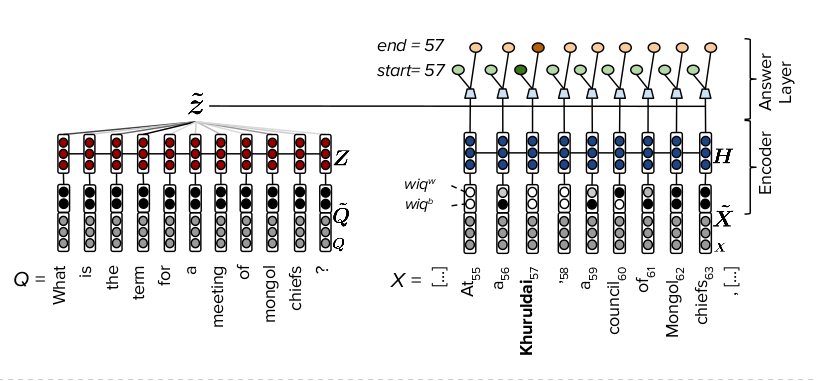
\includegraphics[height=170px]{includes/fast-qa.png}
			\caption{Illustration of FastQA system \et{\citep[Source:][]{fastqa}}}
			\label{fig:fqa}
		\end{figure}

	\end{psubsection}

	\begin{psubsection}{R-Net: Machine Reading Comprehension with Self-Matching Networks}
		R-Net \citep{r-net} is an end-to-end neural network model for reading comprehension and question answering.
		This model consists of four parts:
		\begin{enumerate}
			\item The recurrent network encoder to build representation for questions and passages separately,
			\item the gated matching layer to match the question and passage,
			\item the self-matching layer to aggregate information from the whole passage, and
			\item the pointer-network based answer boundary prediction layer.
		\end{enumerate}

		A view on the R-Net model is given in Figure \ref{fig:r-net}.

		\begin{figure}[ht!]
			\centering
			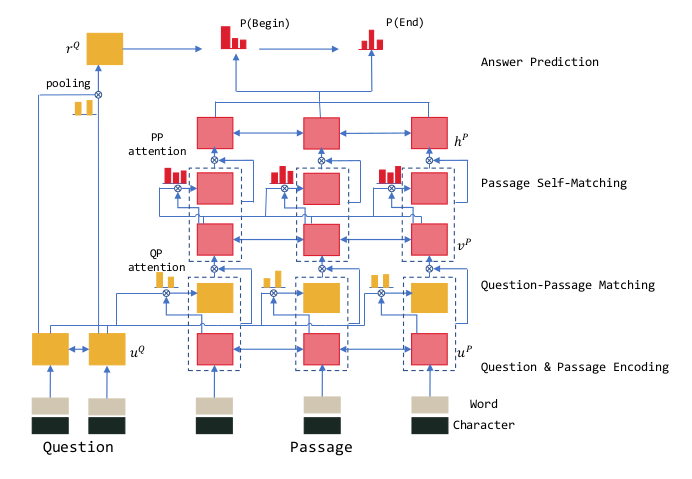
\includegraphics[height=250px]{includes/r-net.png}
			\caption{R-NET structure overview \et{\citep[Source:][]{r-net}}}
			\label{fig:r-net}
		\end{figure}

		\begin{subsubsection}{R-Net Structure}

			\sloppy
			First, the question and passage are processed by a bidirectional recurrent network separately. We then match the question and passage with gated attention-based recurrent networks, obtaining question-aware representation for the passage. On top of that, we apply self-matching attention to aggregate evidence from the whole passage and refine the passage representation, which is then fed into the output layer to predict the boundary of the answer span.

		\end{subsubsection}

		\begin{subsubsection}{Gated Attention Based RNNs}

			A gated attention-based recurrent network is used to incorporate question information into passage representation. It is a variant of attention-based recurrent networks, with an additional gate to determine the importance of information in the passage regarding a question. Different from the gates in LSTM or GRU, the additional gate is based on the current passage word and its attention-pooling vector of the question, which focuses on the relation between the question and current passage word.

		\end{subsubsection}

		\begin{subsubsection}{Self-Matching Attention}

			It is a directly matching the question-aware passage representation against itself. It dynamically collects evidence from the whole passage for words in passage and encodes the evidence relevant to the current passage word and its matching question information into the passage representation. Self-matching extracts evidence from the whole passage according to the current passage word and question information.

		\end{subsubsection}

		\begin{subsubsection}{Output Layer}

			Pointer networks are used to predict the start and end position of the answer. r. In addition, we use an attention-pooling over the question representation to generate the initial hidden vector for the pointer network. Given the passage representation, the attention mechanism is utilized as a pointer to select the start position $p^1$ and end position $p^2$ from the passage.

		\end{subsubsection}

		\sloppy
		The R-Net model is the current state-of-the-art model for machine comprehension on SQuAD. However, we refrain from studying the model due to its complexity and the paper's involved nature.

	\end{psubsection}

	\begin{psubsection}{Question Answering using Match-LSTM and Answer Pointer}

		\cite{match-lstm-mc} introduced the Match-LSTM \citep{match-lstm} model for textual entailment, however, it proved to be useful for the task of machine comprehension as well, with an extra extension using PointerNet \citep{pointernet}.

		In the model proposed by \et{Wang and Jiang}, the architecture consists of three main layers
		\begin{enumerate}[label=\bt{\theenumi.}]
			\ditem[LSTM Preprocessing Layer.]
				The purpose of the \et{LSTM Preprocessing Layer} is to incorporate contextual information into the representation of each token in the passage and the question.
				This is done by passing the passage matrix, $\vP \in \vR^{d \times Q}$ and the question matrix, $\vQ \in \bR^{d \times Q}$ through a one-directional standard LSTM.
				The authors represent this as
				\begin{align*}
					\vH^p	\eq	\overrightarrow{\text{LSTM}}\para{\vP}, \quad\quad
					\vH^q	\eq	\overrightarrow{\text{LSTM}}\para{\vQ}
				\end{align*}
				The matrices $\vH^p$ and $\vH^q$ represent the hidden representations of the passage and the question matrices, respectively.

				\begin{note}
					$Q$ and $P$ are the sizes of or the number of tokens in the question and the passage, respectively
				\end{note}

			\ditem[Match-LSTM Layer.]
				Treating the question as a premise and the passage as the hypothesis, we can apply the Match-LSTM model.
				The model first uses the standard word-by-word attention mechanism to obtain attention weight-vector $\valpha_i \in \bR^Q$ using detailed steps over an additional layer of LSTM. The detailed steps to obtain the attention vector are given in the paper, \cite{match-lstm-mc}.

				This attention is iteratively used to estimate the bidirectional hidden representation of the passage, which in turn is used to compute the attention itself.
				This iterative procedure ensures that the representation we have for the passage is query aware, and is built using the attention obtained from the query (question).
				This representation is denoted by the matrix $\vH^r$

			\ditem[Answer Pointer Layer.]
				The final layer is the \et{Answer Pointer Layer}, which uses the idea of Pointer Networks \cite{pointernet}.
				This model takes in, as input, the hidden representation $\vH^r$, and tries to identify the answer within the passage using two approaches, the \et{sequence model}, which tries to determine the complete sequence and probabilistically models the whole sequence, and the \et{boundary model}, which is only concerned with the starting and ending tokens of the answer. However, we are only interested in the boundary approach, as it performs better, and better suits the nature of PointerNets.

				The passage (hidden representation $\vH^r$) is first passed through the attention mechanism to compute a attention vector $\vbeta_k \in \bR^{P + 1}$, where $\beta_{j, k}$ is the probability of selecting the $j$\tth passage token as the $k$\tth token in the answer. The probability of the answer is then modelled as
				\begin{align*}
					\prob{\va \pipe \vH^r}	\eq	\prob{a_s \pipe \vH^r} \prob{a_e \pipe a_s, \vH^r}
				\end{align*}
				where
				\begin{align*}
					\prob{a_k = j \pipe a_1, a_2 \dots a_{k - 1}, \vH^r}	\eq	\beta_{j, k}
				\end{align*}
				Hence, the objective is to maximize $\prob{\va \pipe \vH^r}$, and the answer corresponding to the maximum answer is reported as the answer to the query.
		\end{enumerate}

		Although the Match-LSTM model works well, the problem with this approach (rather problem with using PointerNets) is that answers which are long, \ie have relatively more number of tokens, are predicted with lesser accuracy. However, one of the key benefits of using Match-LSTM is that it is a simpler model (lesser model complexity) than the other state-of-the-art models, and therefore, might be more scalable than other models.

	\end{psubsection}

	\begin{psubsection}{Comparision of Different Approaches}

		In Table \ref{tab:models}, we have given the EM (Exact Match) and F1 scores \footnote{The description of the scores is given by \cite{squad}}

		\begin{table}[ht!]
			\centering
			\begin{tabular}{l@{\hspace{1em}}|cc|cc}
				\multirow{2}{*}{\bt{Model}}	&	\multicolumn{2}{c|}{\bt{Training Set}}	&	\multicolumn{2}{c}{\bt{Test Set}}	\\
											&	\bt{EM} & \bt{F1}						&	\bt{EM} & \bt{F1}					\\
				\hline
				LR Baseline \citep{squad}	&	40.0 & 51.0								&	40.4 & 51.0							\\
				BiDAF \citep{bidaf}			&	68.0 & 77.3								&	68.0 & 77.3							\\
				FastQA \citep{fastqa}		&	-	 & -								&	68.4 & 77.1							\\
				R-Net \citep{r-net}			&	72.3 & 80.6								&	72.3 & 80.7							\\
				Match-LSTM \citep{match-lstm-mc}	&	64.1 & 73.9						&	64.7 & 73.7							\\
			\end{tabular}
			\caption{Comparision of different models for Machine Comprehension \et{\citep[Source:][]{r-net}}}
			\label{tab:models}
		\end{table}

		\note{The scores are given for single models only, and do not involve ensembles, however for most models, ensembles perform better that single models.}

	\end{psubsection}

\end{psection}

\begin{psection}{Goals of the Project}

	In our project, we will explore the various approaches that have been used for machine comprehension, and try to study the scalability and the performance of each model. The problem with most approaches discussed is the low speed of convergence, given the enormous number of weights in the models.

	We’ll try to adopt model compression based on removing redundant structure in original DNNs \citep{iss}, to provide scalability and wide adoption corresponding to limited resources. We will attempt to extend the Match-LSTM and Answer-Pointer model used by \et{Wang and Jiang}, considering it is a relatively simple model, and apply Sparsity Reduction on them, hoping to significantly reduce the training time, and to make the model simpler.

	Pruning approaches produce non-structurally sparse LSTMs which provide comparatively lower speedups in comparison to structurally sparse lstms. A visual comparision is given in \ref{fig:iss-graph}. Therefore we’ll use group lasso regularization in order to obtain structurally sparse LSTMs, as explained by \cite{iss}. It can both reduce parameters in models and obtain regular nonzero weights for fast computation
	(non structural / irregular pattern of non-zero weights may not be friendly for computation efficiency.)

	We also aim to reduce the number of basic structures simultaneously during learning such that the original schematic and dense structure of the lstms are retained along with reducing sizes of these basic structure.

	To start we’ll try to Identify structure inside the LSTMs that shall be considered as a group to most effectively explore sparsity in these basic structure. The basic structures interweave with each other, independently removing these structures can result in mismatch of their dimensions and then inducing invalid recurrent units. Therefore to deal with this we include Intrinsic Sparse Structure within LSTMs.

	To learn sparse ISS, we turn to weight sparsifying. We can remove one component of ISS by zeroing out all associated weights, lets say k-th hidden state of h is removable, now all the connection receiving these stages can be removed. However, the number of weights in one ISS weight group can be very large, for avoiding overfitting and maintaining original recognition we can independently sparsify each weight using l1-norm regularization. Decreasing the size of ISS simultaneously reduce the dimensions of basic structures.

	\begin{figure}[ht!]
		\centering
		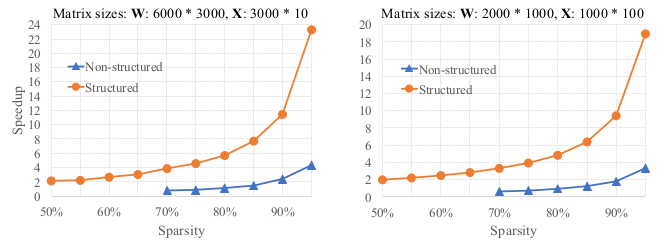
\includegraphics[height=170px]{includes/iss-graph.png}
		\caption{Speedups of Matrix Multiplication using Non-Structured and Sparsity \et{\citep[Source:][]{iss}}}
		\label{fig:iss-graph}
	\end{figure}

	\et{Wen et al.} have explained this pruning technique in detail in their paper, where they analyze the BiDAF model \citep{bidaf}. We wish to explore the application of the same approach on a heavier and simpler model, and find the trade off between the performance drop, and the speed boost.

	If time allows, we will explore further extensions to the model, such as exploring techniques to find better word embeddings, to allow more information embedding in the word vectors, for example, including the genre of the passage provided to us, or adding semantic features within the word embeddings.

	Another problem with Match-LSTMs (which R-Net handles efficiently) is that all question types have the same attention mechanism.If time allows, we will also look into tweaking the model to deal with different types of questions differently, particularly tweaks in the attention mechanism, \ie for different question types, such as `Why?', `What?', etc.
	This is relevant as different question types demand different format of the answers, for example a `Who?' question would focus more on the subject or the object of the sentence. This might increase the performance of the Match-LSTM model, however, will also add to the complexity of the model, and therefore the training time.

\end{psection}

\newpage

\bibliography{proposal}
\bibliographystyle{plainnat}

\end{document}
